\section{Sécurité}

\subsection{Contrôle d'accès}
Cette application web est destinée à être utilisée par plusieurs personnes avec des rôles différents au sein de la société. Chaque rôle n'a pas les mêmes droit quant à la consultation ou manipulation des données de l'application. On peut ainsi distinguer cinq catégories d'utilisateurs: 
\begin{enumerate}
  \item \textbf{Inconnu}: utilisateur non-authentifié. Celui-ci n'a aucun droit sur les données et peut uniquement accèder à la page de connexion de l'application. 
  \item \textbf{Comptabilité}: 
  \begin{itemize}
    \item a tous les droits de l'inconnu
    \item peut uniquement consulter l'ensemble des données 
    \item peut générer des pdf (factures, commandes, ...)
  \end{itemize}
  \item \textbf{Atelier}: 
  \begin{itemize}
    \item a tous les droits de la comptabilité
    \item peut créer/modifier une fiche de Travail
    \item peut créer/modifier une commande
  \end{itemize}
  \item \textbf{Administration}: 
  \begin{itemize}
    \item peut tout faire hormis supprimer les utilisateurs de type "Développeur"
  \end{itemize}
  \item \textbf{Développeur}: 
  \begin{itemize}
    \item peut tout faire et a accès aux logs et métriques
  \end{itemize}
\end{enumerate}

\newpara

Afin d'authentifier un utilisateur et donc de lui donner certain droits ou non, l'application utilise des JSON Web Tokens (JWT)\footnote{Comment cela fonctionne-t-il? Explication en vidéo: \url{https://www.youtube.com/watch?v=7Q17ubqLfaM}}. Les tokens sont générer lors de chaque nouvelle connexion réussie et sont valide pendant 48h. Toute action effectuée à l'aide d'un token non-valide déconnecte automatiquement l'utilisateur et le re-dirige vers la page de connexion. 

\newpage

\subsection{Hachage et Chiffrement}

Avant toute choses il me semble bon de rappeler la différence entre le \textbf{hachage} et le \textbf{chiffrement}: 
\begin{itemize}
  \item \textbf{hachager}: \\ Utilisation d'un algorythme de hachage uni-directionnel afin de transformer les données de manière irréversible et de longueur fixe. Il est donc possible de comparé deux hash.
  \item \textbf{chiffrer}: \\ Encoder des données afin qu'uniquement la personne ayant la clé de déchiffrement puisse les déchiffrer. Cette action est donc réversible.
\end{itemize}

\subsubsection{Données enregistrées}
Toute donnée susceptible d'être un risque pour l'intégrité et la protection de l'application ou des autres données est stockée sous forme de hash (et non en clair\footnote{lisible et comprehensible par quiconque}) dans la base de donnée (par exemple les mots de passes des utilisateurs). 

\newpara

Afin de hasher ces données, j'ai utilisé la librairie "bcrypt". La librairie "bcrypt" est une des librairies de hashage les plus réputées. Elle permet d'incorporer un sel (salt)\footnote{\textit{"Le salage, est une méthode permettant de renforcer la sécurité des informations qui sont destinées à être hachées (par exemple des mots de passe) en y ajoutant une donnée supplémentaire afin d’empêcher que deux informations identiques conduisent à la même empreinte (la résultante d’une fonction de hachage)"}\cite{Salt}} afin de se protéger contre les attaques par table de correspondance (rainbow table)\footnote{Attaque consistant à comparer un hash à un table reprenant un grand nombre de paires de text clair et le hash correspondant.}. De plus elle est facilement paramétrable permettant ainsi d'augmenter la complexité de l'algorithme utilisé afin de palier aux attaques par force brute\footnote{Attaque consistant à essayer un grand nombre de donnés générées automatiquement en espérant trouver la bonne.} utilisant des machines à puissances de calcule importante. 

\subsubsection{HTTPS}
Stocker les données à risque de manière chiffrée dans la base de donnée est une chose, cependant, avant que les données n'arrivent jusque là elles sont potentiellement envoyées en clair sur le réseau (internet). Afin d'éviter cela, je n'autorise que les connexion HTTPS et redirige les connexions HTTP vers le HTTPS. Ceci permet de garantir que l'entièreté des données envoyées sont chiffrées et dès lors beaucoup moins vulnérables aux attaques de type "Man In The Middle" (MITM).

\newpage

\subsection{Security Headers}
\begin{figure}[H]
  \centering
  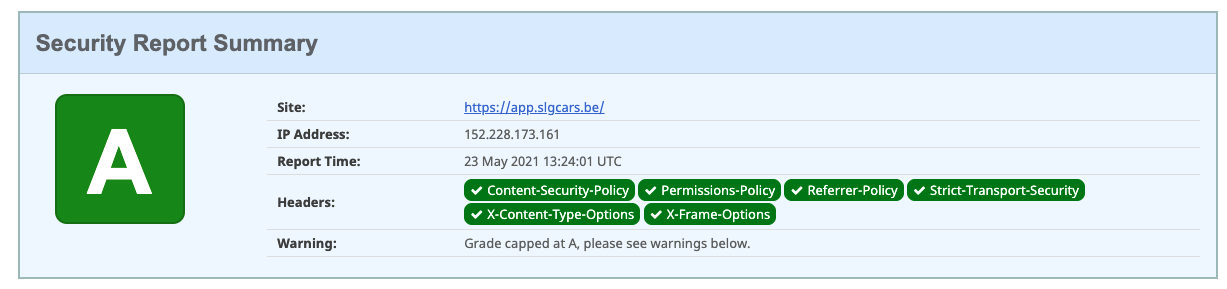
\includegraphics[width=\linewidth]{img/securityHeaders.png}
  \caption{Résultat analyse de sécurité des headers fait sur \url{https://securityheaders.com/}}
\end{figure}

\subsection{Dependabot Github}
\begin{figure}[H]
  \centering
  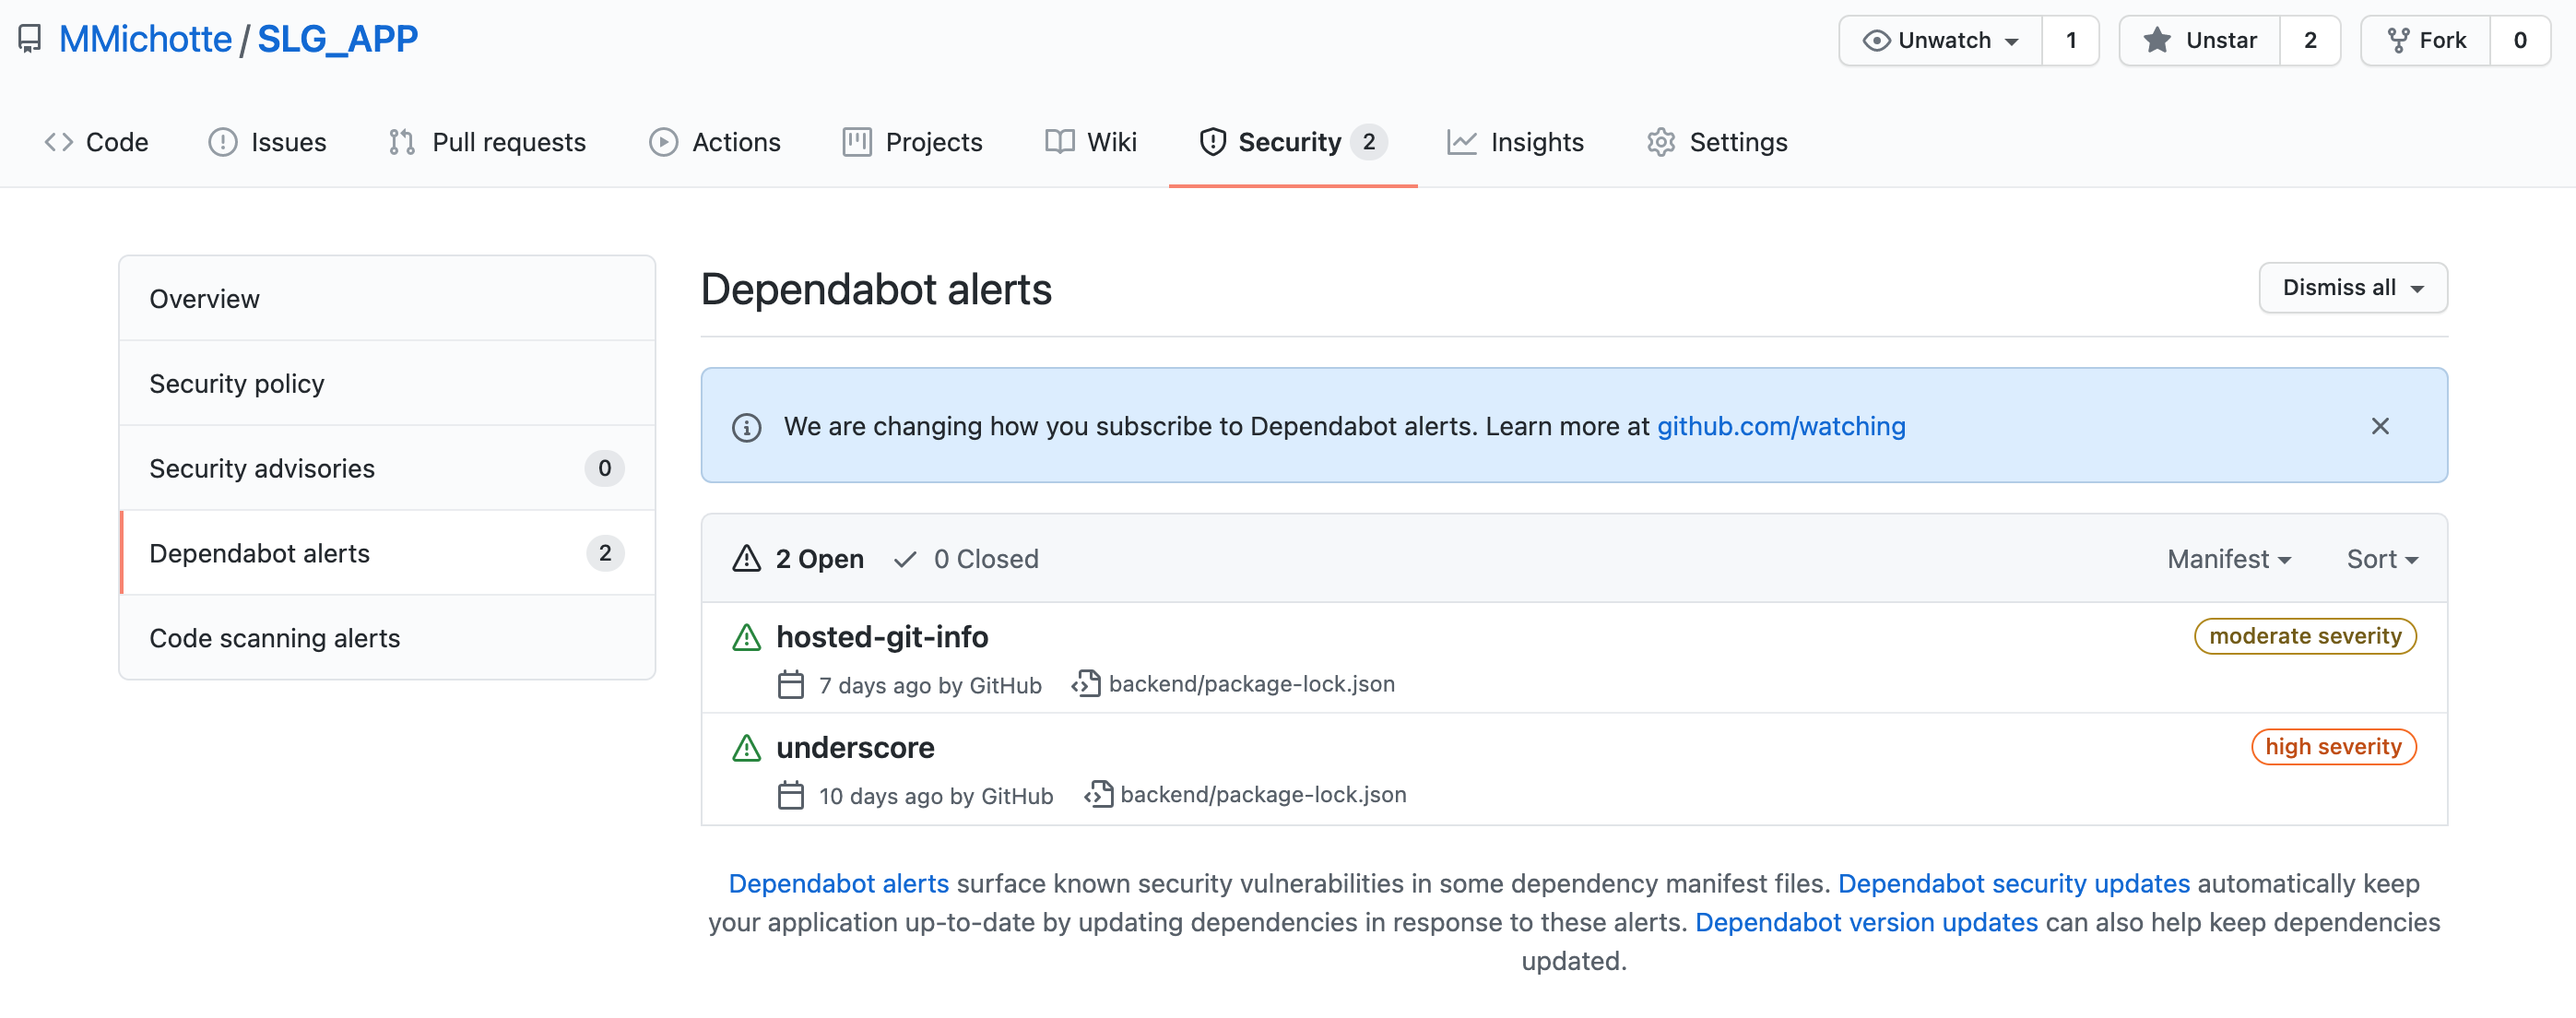
\includegraphics[width=\linewidth]{img/dependabot.png}
  \caption{Alertes générées par "Dependabot"}
\end{figure}